\documentclass[11pt]{article}
\usepackage[utf8]{inputenc}
\usepackage{amsmath,amssymb}
\usepackage{graphicx}
\usepackage{booktabs}
\usepackage{authblk}
\usepackage[margin=1in]{geometry}
\usepackage[hidelinks]{hyperref}

\title{RealNucleus: Nuclear Binding as Dual Coulomb Confinement,\\ without a Strong or Weak Force}

\author[1]{Claes Johnson}
\affil[1]{KTH Royal Institute of Technology, Stockholm, Sweden \\
\texttt{claesjohnson@gmail.com}}
\date{\today \\[0.4em]
\small\textit{Mathematical formulation by the author; implementation developed} \\
\small\textit{with AI assistance (Claude, Anthropic).}}

\begin{document}
\maketitle

\begin{abstract}
\textbf{RealQM} is a parameter-free, real-space model of quantum mechanics in which charge
appears as a sum $\Psi=\sum_i\psi_i$ of one-particle components, each carrying unit charge on a
non-overlapping domain separated by free boundaries, the ground state minimising the
\emph{Coulomb} energy over components and partition~\cite{Johnson-RealQM,Johnson-Book,Johnson-Atoms}.
We carry this model into the \textbf{atomic nucleus} through the proton--electron picture,
treating protons and electrons as the \emph{same} object --- equal-mass charge clouds
differing only in the \emph{sign} of the charge --- interacting through \textbf{Coulomb forces
only}, with \textbf{no strong force}. Binding is by \textbf{dual confinement}: the electron
clouds hold the protons together against their repulsion while the protons cage the electrons
against theirs. Calibrating one energy scale on the deuteron ($2.22$~MeV), the alpha emerges at
\textbf{103\%} of its experimental binding with no fitting (alpha/deuteron ratio $13.1$ versus
$12.7$), and the ladder $^2\mathrm{H}\to{}^4\mathrm{He}\to{}^8\mathrm{Be}\to{}^{16}\mathrm{O}$
binds as \emph{single} connected units with near-constant binding per nucleon (saturation) as the
nucleus adds shells. No \emph{weak} force is needed either: the model ``neutron''
($\mathrm{1p}+\mathrm{1e}$) is computed \emph{unbound}, so free-neutron $\beta$-decay into a
proton and an electron follows from the same Coulomb energetics. The model is solved by signed
Poisson and free-boundary evolution on a GPU and runs in a web browser.

\medskip
\noindent\textbf{Keywords:} nuclear binding; proton--electron model; Coulomb confinement;
real-space methods; multiphase wave functions; free-boundary problems; alpha clustering;
strong force; weak force; beta decay.
\end{abstract}

\section{Introduction}

For ninety years it has been a fixed point of physics that the atomic nucleus cannot be held
together by electromagnetism. The protons are all positively charged and repel; something else,
a short-range \emph{strong} force --- mesons in Yukawa's formulation, residual QCD today --- must
overcome that repulsion. This force is one of the four fundamental interactions, and the whole of
nuclear physics since Chadwick's neutron in 1932 rests on it. To propose that a nucleus is bound
by Coulomb forces \emph{alone}, with no strong force at all, therefore looks not merely wrong but
impossible: it is the textbook reason the strong force had to be invented.

This article nonetheless asks exactly that question --- and reports a computation that, to our
own surprise, answers it in the affirmative for the light nuclei. The move that reopens the
question is to abandon the point-particle, protons-and-neutrons description and return to the
older \emph{proton--electron picture} of the nucleus, but with protons and electrons represented
as \emph{charge clouds} in the manner of RealQM. We then ask: does the ordinary Coulomb
interaction, with no separate strong force, already account for nuclear binding?

The proton--electron picture takes a neutron to be a bound proton--electron pair
($n = p + e$), consistent with $\beta$-decay $n\to p+e+\bar\nu$. A nucleus of mass number $A$
and atomic number $Z$ then consists of $A$ protons and $A-Z$ electrons. The deuteron
($^2\mathrm{H}=\mathrm{p}+\mathrm{n}$) is $\mathrm{2p}+\mathrm{1e}$; the alpha
($^4\mathrm{He}=\mathrm{2p}+\mathrm{2n}$) is $\mathrm{4p}+\mathrm{2e}$; oxygen-16 is
$\mathrm{16p}+\mathrm{8e}$.

In RealQM~\cite{Johnson-RealQM,Johnson-Atoms} charge is carried by one-particle components on
\emph{non-overlapping} spatial domains, with continuity and Bernoulli (pressure-balance)
conditions across the free boundaries between them. Non-overlap takes the place of
antisymmetry and the exclusion principle; there is no determinant and no spin. We apply this
model to the nucleus with one essential symmetrisation: protons and electrons are treated as
the same kind of object --- equal-mass charge clouds --- so that the only distinction between
them is the sign of their charge. The interaction is Coulomb and nothing else.

The mechanism that emerges we call \textbf{dual confinement}. A single electron placed between
two protons binds them: its negative cloud sits in the region where it most lowers the energy,
between the two positive clouds, and holds them against their mutual repulsion --- this is the
deuteron, and it is the same mechanism that binds the one-electron molecular ion
$\mathrm{H}_2^+$. Reciprocally, the two protons confine the electron, which would otherwise
spread away. In a larger nucleus the same balance operates on both species at once: the
electron clouds keep the protons from flying off, and the proton clouds keep the electron
clouds together. The nucleus is a self-confined two-component Coulomb system, stabilised by the
RealQM non-overlap condition.

We report that this purely electromagnetic packing reproduces the scale and trends of nuclear
binding. The central claim of the paper is therefore the title's: \textbf{nuclear binding is
dual Coulomb confinement of proton and electron charge clouds, and no strong force is needed},
neither for the binding itself nor for the saturation (constant binding per nucleon) of larger
nuclei.

\section{The model}

\subsection{Energy and the dual-confinement functional}

The state is a finite family of real one-particle components $\{\psi_i\}$, each supported on
its own domain $\Omega_i$, with the $\Omega_i$ tiling space without overlap. Component $i$
carries a signed charge density $\rho_i = q_i\,\psi_i^2$ with $q_i=+1$ for a proton cloud and
$q_i=-1$ for an electron cloud. With equal masses $m_i\equiv m$ the energy is the standard
kinetic-plus-Coulomb functional
\begin{equation}
E[\{\psi_i\},\{\Omega_i\}]
 \;=\; \sum_i \frac{1}{2m}\int_{\Omega_i}|\nabla\psi_i|^2
 \;+\; \frac12\iint \frac{\rho(x)\,\rho(x')}{|x-x'|}\,dx\,dx',
 \qquad \rho=\sum_i \rho_i ,
\label{eq:energy}
\end{equation}
to be minimised over the components (normalised on their domains) \emph{and} over the partition
$\{\Omega_i\}$. The Coulomb term is evaluated by a Poisson solve for the potential of the
signed density $\rho$. The interfaces between domains are \emph{free boundaries}, located by
the Bernoulli condition that the energy be stationary under moving the interface (balance of
the normal-derivative/pressure jump). Crucially, \textbf{this is the \emph{same} condition on
\emph{every} interface} --- electron--electron, electron--proton, and proton--proton alike ---
exactly as in the atomic RealQM model~\cite{Johnson-Atoms}, where only electron--electron
interfaces occur. The sign of the charge enters only through the Coulomb term; the boundary
law itself does not distinguish proton from electron. There is no strong-force term, no spin,
and no exclusion beyond non-overlap.

The two signs in $q_i$ are the whole of the physics. The cross terms $q_iq_j<0$ between proton
and electron clouds are \emph{attractive} and do the binding; the like-sign terms $q_iq_j>0$
(proton--proton and electron--electron) are repulsive. Dual confinement is the statement that,
in the minimising partition, every proton cloud is wrapped by enough electron density that the
attractive cross terms outweigh the proton--proton repulsion, and vice versa. Binding is
measured against the fully separated constituents (all clouds pulled infinitely apart, energy
zero); a negative $E$ is a bound nucleus.

\subsection{How dual confinement is possible}

That two species of like-repelling charges could hold \emph{each other} together can seem
miraculous. A short chain of familiar facts makes it plausible. Begin with hydrogen: one proton
binds one electron. The negative ion $\mathrm{H}^-$ --- one proton with \emph{two} electrons ---
is a stable, bound configuration; so a single proton already holds \emph{two} electrons together
against their mutual repulsion. Now exchange the roles of the two charges, which the equal-mass,
sign-only model permits: by the same token a single electron should be able to bind \emph{two}
protons around it. Iterating, a core of $Z$ electrons can bind $2Z$ protons around it. This is one
half of the dual confinement --- the half in which the electron core holds the protons in.

What remains is the other half: that the $2Z$ protons, arranged as a shell surrounding the
electron core, act as a \emph{cage} that keeps the electrons together despite their mutual
repulsion. A surrounding shell of positive charge is exactly such a cage --- it draws every inner
electron outward toward the shell and so prevents the negative core from dispersing, just as the
inner electrons draw the shell inward. The two confinements are not two mechanisms but one Coulomb
attraction read from the two sides. Seen this way, a nucleus held together without a strong force
is $\mathrm{H}^-$ and its role-reversed image, iterated and caged: what looks like a miracle need
not be miraculous.

The electron glue, however, cannot be spherically symmetric --- the central structural fact of
the model. It must break spherical symmetry to interpenetrate the protons; a spherically
symmetric electron core, held at distance from the protons it should bind, does not. This is an
empirical statement, not an idealisation: the fully spherical configuration --- a homogeneous
$-2$ core inside a homogeneous $+4$ shell, even with reduced self-repulsion --- does not bind
(\S4.1, Table~\ref{tab:symmetry}), whereas the binding switches on the moment the electron core
is split, and is already substantial for the minimal split into two halfspaces. The proton and
electron potentials (Fig.~\ref{fig:confinement}) are correspondingly structured rather than
featureless: the proton potential is peaked toward the centre where the electron core sits, the
electron potential a deep central well into which the protons are drawn. The two species are held
only by each other.

\begin{figure}[t]
\centering
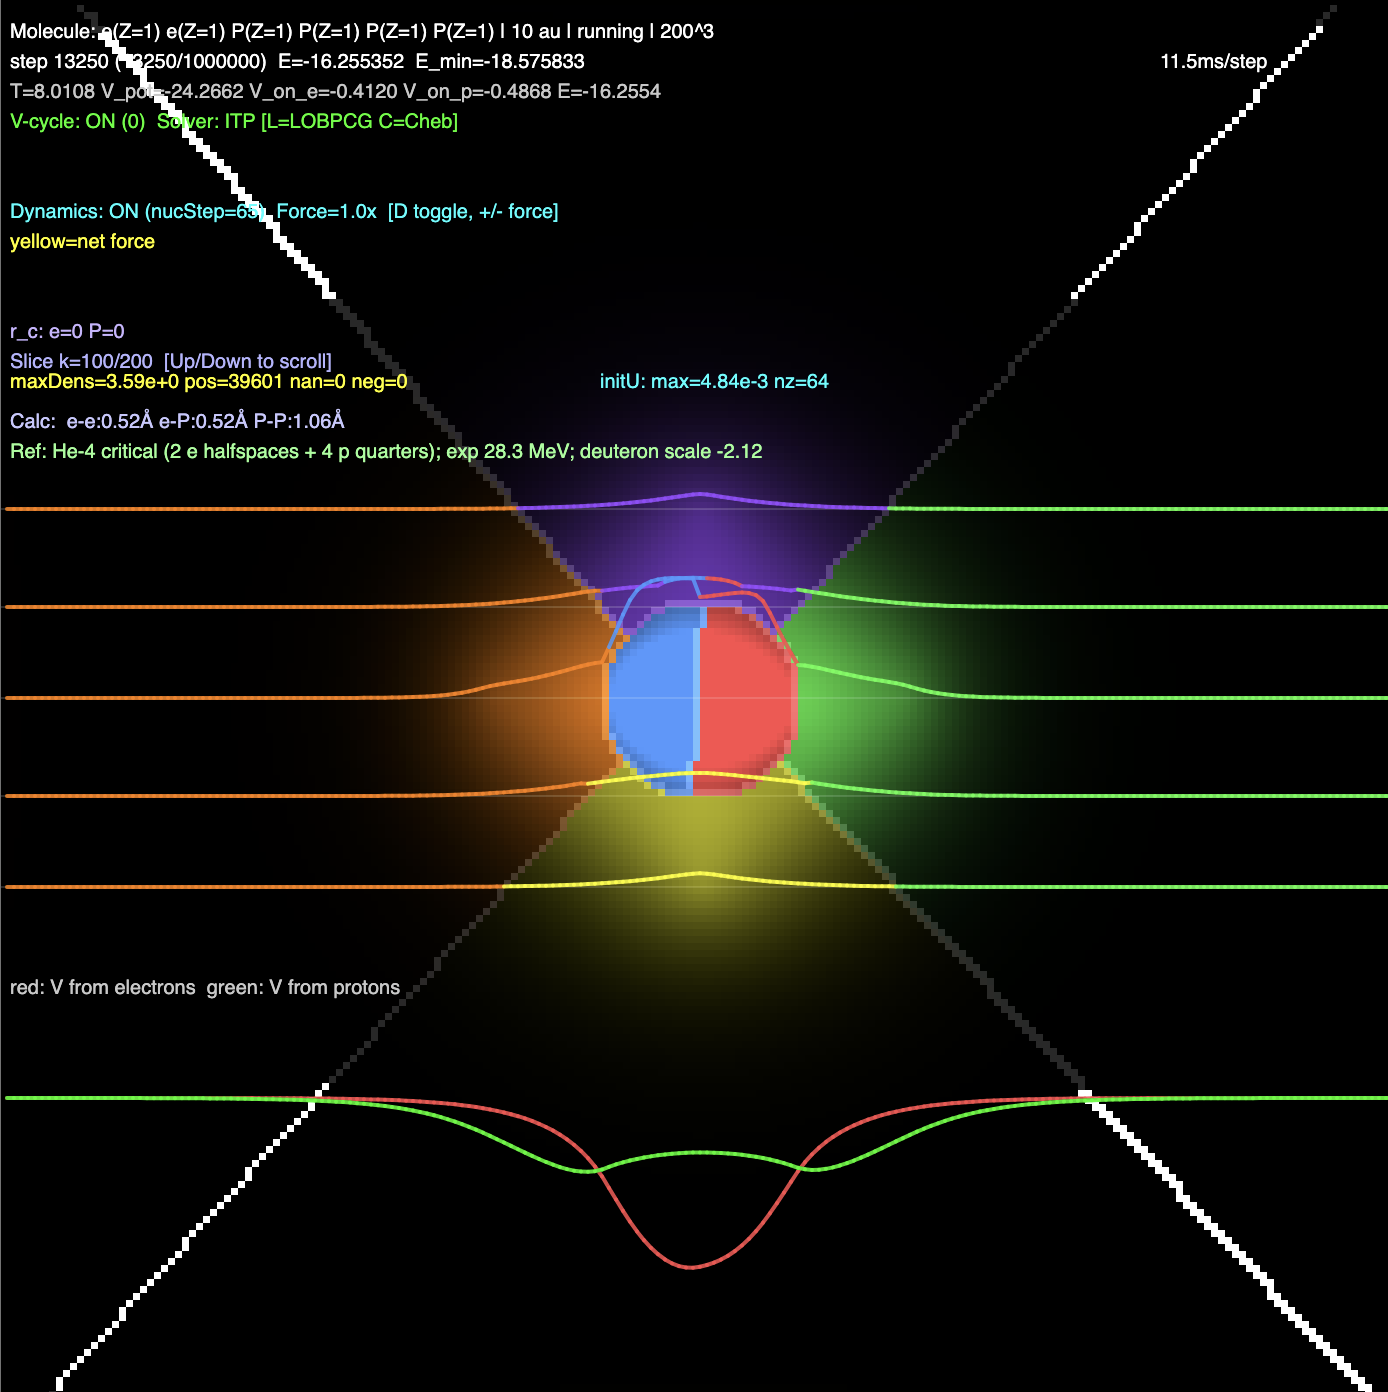
\includegraphics[width=0.72\textwidth]{confinement22e4p.png}
\caption{Dual confinement in He-4 (the minimal-break configuration, $E=-18.5$, $69\%$ of
experiment; cf.\ Table~\ref{tab:symmetry}). An inner core of two electrons, split into
half-spheres, generates the red potential --- a deep central well that draws the four protons
inward. The four protons, split into quarter-spaces, generate the green potential that cages the
electron core from outside. Each species is held only by the other's Coulomb potential (legend:
red $=V$ from electrons, green $=V$ from protons).}
\label{fig:confinement}
\end{figure}

\subsection{Why no neutron core, and why no collapse}
\label{sec:neutron}

Two consistency checks frame the model. First, a single proton--electron pair
($\mathrm{1p}+\mathrm{1e}$, the model ``neutron'') is found \emph{unbound} on its own: with no
second proton to share, the electron cannot lower the energy below the separated state. This
matches the instability of the free neutron and fixes the binding reference as free protons and
electrons, not free neutrons. Second, the clouds do not collapse onto one another despite the
attractive cross terms, for exactly the reason a hydrogen atom does not collapse: the kinetic
energy in~\eqref{eq:energy} rises as $1/(\text{size})^2$ under compression and overwhelms the
$1/(\text{size})$ Coulomb gain. Stability of size is thus electromagnetic and kinetic, of the
same origin as atomic stability.

\section{Method}

The functional~\eqref{eq:energy} is minimised by three coupled flows, as in
RealQM~\cite{Johnson-RealQM}: imaginary-time propagation of each one-particle component,
a (signed) Poisson solve for the Coulomb potential, and free-boundary evolution of the
partition. The computation is carried out in 3D on a Cartesian grid with a WebGPU solver; the
signed-charge Poisson equation and the level-set partition are the only changes from the atomic
solver. Protons and electrons are assigned equal mass, so both render as genuine charge clouds
(a physical-mass proton, $1836\times$ heavier, would localise to a near-point and obscure the
picture without changing the qualitative balance).

Nuclei are built as nested shells: electron clouds occupy inner shells, proton clouds the outer
shells, the radial partition assigning each spherical zone to its component. A shell of $n$
clouds is seeded as $n$ symmetric points ($n=2,4,8$: an opposed pair, a tetrahedron, a cube),
which the partition renders as a spherical shell ($n=1$) or an angularly split shell. We write
a configuration as \emph{electron-shells} $\mid$ \emph{proton-shells} from inner to outer; e.g.
$2{+}2\mid 4{+}4$ is two electron pairs inside two proton quartets. Energies are reported in a
model unit fixed once, on the deuteron.

\section{Results}

\subsection{The light nuclei and the single calibration}

Table~\ref{tab:ladder} collects the ladder. One scale is set by the deuteron,
$E(^2\mathrm{H})=-2.12$ model units $\leftrightarrow 2.22$~MeV; everything else follows with no
further fitting. The alpha particle is $\mathrm{4p}+\mathrm{2e}$, and its main configuration is
the dual-confined structure of Fig.~\ref{fig:confinement}: the two electrons split into halfspaces
forming the $-2$ glue, the four protons into quarter pieces. The role of the broken spherical
symmetry is direct and decisive (Table~\ref{tab:symmetry}). The fully spherical configuration ---
a homogeneous $-2$ core inside a homogeneous $+4$ shell, \emph{even with reduced self-repulsion}
--- does not bind ($E\approx 0$): by the shell theorem a spherical proton shell exerts no force on
the electrons it encloses. The minimal break of that symmetry --- the two electron halfspaces
gluing the four proton quarters --- already recovers most of the binding ($E=-18.5$, $69\%$ of
experiment). Concentrating the glue optimally, as a $-2$ core in a nested $2{+}2$ proton
arrangement, then sharpens it to $E=-27.8$, i.e. \textbf{29.1~MeV against the experimental 28.3
(103\%)}, with the alpha/deuteron ratio $13.1$ versus the experimental $12.7$. That a single
Coulomb scale carries the most tightly bound light nucleus with no adjustable parameter is the
central quantitative result.

\begin{table}[t]
\centering
\begin{tabular}{lllr}
\toprule
electron symmetry & alpha configuration & $E$ (model) & \% exp.\\
\midrule
spherical & homogeneous $-2$ core $+$ $+4$ shell & $\approx 0$ & $0\%$\\
minimal break & 2 halfspaces $+$ 4 quarters & $-18.5$ & $69\%$\\
optimal & $-2$ core, nested $2{+}2$ protons & $-27.8$ & $103\%$\\
\bottomrule
\end{tabular}
\caption{The alpha binds only when the electron glue breaks spherical symmetry. A fully spherical
configuration (homogeneous core and shell, reduced self-repulsion) does not bind; the minimal
halfspace split recovers most of the binding; optimal concentration of the glue reaches
experiment. One scale throughout, fixed on the deuteron.}
\label{tab:symmetry}
\end{table}

This alpha binding is also the energy of \emph{fusion}: the ${\sim}28$~MeV liberated when four
protons and two electrons assemble into $^4$He is what powers the stars and is the goal of
controlled fusion, and here it is simply the Coulomb binding released as the proton and electron
clouds lock into the dual-confined alpha. The assembly of the alpha from hydrogen is treated more
fully in the monograph~\cite{Johnson-Book} and the interactive gallery~\cite{Gallery}.

\begin{table}[t]
\centering
\begin{tabular}{llrrr}
\toprule
nucleus & structure (e $\mid$ p) & $E$ (model) & MeV & \% exp.\\
\midrule
$^2$H  & $1\mid 2$            & $-2.12$ & $2.22$  & calib.\\
$^4$He & $2\mid 4$ (core)     & $-27.8$ & $29.1$  & 103\%\\
$^8$Be & $2{+}2\mid 4{+}4$    & $-58$   & $61$    & 108\%\\
$^{16}$O & $2{+}2{+}2{+}2\mid 4{+}4{+}4{+}4$ & $-129$ to $-138$ & $135$--$144$ & 106--113\%\\
\bottomrule
\end{tabular}
\caption{The RealNucleus ladder. One scale fixed on the deuteron
($-2.12\leftrightarrow 2.22$~MeV); all other entries follow with no fitting. Experimental
bindings: $^2$H 2.22, $^4$He 28.3, $^8$Be 56.5, $^{16}$O 127.6~MeV.}
\label{tab:ladder}
\end{table}

\subsection{Binding as a single connected unit, not as separated clusters}

Every member of the ladder binds as a \emph{single} dual-confined Coulomb unit, the proton and
electron clouds wrapping one another throughout. The alpha appears only as a \emph{compositional}
motif --- each $(\mathrm{2e}+\mathrm{4p})$ group is a confined sub-unit and $^{16}$O is built of
four of them --- but \emph{spatially} the lowest-energy form is a single connected structure
(the nested $2{+}2{+}2{+}2\mid 4{+}4{+}4{+}4$ shells of \S4.3), not four separated alpha
droplets. The two are not equivalent in the model, and the difference is decisive: assembling
$^{16}$O as four \emph{spatially separated} alpha clusters leaves each cluster with net charge
$+2$, so the clusters repel and the separated arrangement binds only ${\sim}82\%$ of experiment
--- \emph{below} the connected unit and below even the sum of four free alphas. \textbf{The model
therefore disfavors separate clustering in $^{16}$O}: the nucleus is one mutually-confined cloud
system, more bound than its parts held apart, and there is no preferred tetrahedral four-droplet
ground state. The single exception is $^8$Be, which the model finds only \emph{marginally} bound
as two near-touching alphas --- matching the empirical fact that $^8$Be is unstable and decays
into two alpha particles. Across the experiment-matching connected configurations the binding
tracks ${\sim}7$~MeV per nucleon, the empirical volume law, reflecting the roughly constant
density that the shell count enforces (\S4.3).

\subsection{Electron concentration sets the binding; shell spread sets saturation}

A systematic scan over shell configurations at fixed radial spacing shows a single controlling
variable: the \emph{concentration of the electron glue}. Concentrated electron cores over-bind,
diffuse cores under-bind, and an intermediate concentration matches experiment. For $^8$Be the
electron arrangement $4\to 2{+}2\to 1{+}1{+}1{+}1$ runs the binding from $153\%$ through $108\%$
down to $68\%$ of experiment, with $2{+}2$ on target.

The over-binding of the most \emph{compact} large configurations is removed without any new
force: as a nucleus grows it \emph{adds shells}, spreading the charge. For $^{16}$O, spreading
the electrons from two shells ($4{+}4$, $177\%$) to four shells ($2{+}2{+}2{+}2$) brings the
binding down to $106$--$108\%$ of experiment (Table~\ref{tab:ladder}). The shell count, set by
the nucleon count, fixes the size and hence the density --- this is the nuclear
\emph{saturation}, and it too is purely structural and electromagnetic. The winning
$^{16}$O structure, $2{+}2{+}2{+}2\mid 4{+}4{+}4{+}4$, is exactly four nested
$(\mathrm{2e}+\mathrm{4p})$ alpha-units arranged as concentric shells.

\subsection{Binding per nucleon and saturation}
\label{sec:perA}

The matched packing extends to a single ladder built by \emph{adding one
$(\mathrm{2e}+\mathrm{4p})$ alpha-unit at a time}, electron pairs inside, proton quartets
outside (Table~\ref{tab:perA}). The result is the empirical hallmark of nuclear binding:
\textbf{binding per nucleon is essentially constant} along the ladder. From $^8$Be onward the
model sits at a uniform $107$--$108\%$ of experiment, and its binding per nucleon
($7.5\to8.2\to8.6$~MeV) even \emph{tracks the experimental rise} toward the iron peak
($7.1\to7.7\to8.0$). Each added alpha-unit contributes a near-constant binding --- saturation,
emerging from dual Coulomb confinement with one scale and no fitting.

\begin{table}[t]
\centering
\begin{tabular}{llrrr}
\toprule
nucleus & pattern (e $\mid$ p) & $E$ (model) & MeV/$A$ & \% exp.\\
\midrule
$^2$H   & $1\mid 2$                              & $-2.12$ & $1.1$  & calib.\\
$^4$He  & $2\mid 4$                              & $-19.4$ & $5.1$  & 72\%\\
$^8$Be  & $2{+}2\mid 4{+}4$                      & $-57.6$ & $7.5$  & 107\%\\
$^{12}$C& $2{+}2{+}2\mid 4{+}4{+}4$              & $-94.3$ & $8.2$  & 107\%\\
$^{16}$O& $2{+}2{+}2{+}2\mid 4{+}4{+}4{+}4$      & $-132.1$& $8.6$  & 108\%\\
\bottomrule
\end{tabular}
\caption{Binding per nucleon along the matched alpha-unit ladder (one scale fixed on
$^2$H). From $^8$Be on, the model holds a uniform $107$--$108\%$ of experiment with nearly
constant MeV/$A$ --- saturation. Experimental MeV/$A$: $^4$He 7.07, $^8$Be 7.06, $^{12}$C 7.68,
$^{16}$O 7.98.}
\label{tab:perA}
\end{table}

Two members sit apart from the trend, both correctly. $^4$He, the single alpha-unit, is the
lone outlier at this fixed spacing ($72\%$); being the smallest and densest nucleus it wants a
tighter size, and given it returns $103\%$ (\S4.1) --- so the \emph{one}-unit member needs its
own scale while every multi-unit member falls on the pattern. The deuteron ($1\mid2$) is the
anchor and, like the real deuteron, is anomalously weakly bound and does not follow the
per-nucleon trend.

\paragraph{Extrapolation.} Because each $(\mathrm{2e}+\mathrm{4p})$ unit adds a near-constant
binding, \emph{continuing the pattern} --- $2{+}2{+}2{+}2{+}2\mid 4{+}4{+}4{+}4{+}4$ for
$^{20}$Ne, and so on --- is expected to keep MeV/$A$ flat at the saturated value. We state this
as a conjecture: the dual-confinement ladder should reproduce the flat plateau of the nuclear
binding curve for the alpha-conjugate nuclei, with the slow rise toward the iron peak coming
from the same gentle trend already visible in Table~\ref{tab:perA}. Direct confirmation beyond
$^{16}$O requires computation at larger nucleon number; we leave the heavier alpha-conjugate
nuclei, and the magic numbers $20$ and beyond, to future work.

\section{Discussion: no strong force, and no weak force}

The results support a single, deliberately strong claim: \textbf{nuclear binding is the dual
Coulomb confinement of proton and electron charge clouds, and a strong force is not required.}
The evidence is that (i)~the deuteron and the alpha bind \emph{quantitatively} from one Coulomb
scale; (ii)~the whole light ladder binds as single connected dual-confined units --- with the
volume law emerging and $^8$Be left only marginally bound against alpha breakup, as observed;
and (iii)~the saturation of larger nuclei follows from the shell
structure spreading with nucleon number, requiring no short-range repulsive core. At no point is
a strong-force term present in~\eqref{eq:energy}; the only interaction is Coulomb, and the only
structural rule is non-overlap.

The conventional motivation for the strong force --- that like-charged protons cannot bind ---
is dissolved by the proton--electron picture: the nucleus is not a collection of protons only
but a two-component Coulomb system in which the electron clouds supply the binding and the
proton clouds the confinement, mutually. The neutron is not an elementary neutral particle to be
glued in, but a proton locally confined by an electron; ``the strong force'' is, on this view,
the effective name for the Coulomb confinement that the proton--electron clouds already provide.

\subsection{Relation to earlier nuclear models}

The picture used here is, in outline, an old one. After Rutherford's nuclear
atom~\cite{Rutherford1911}, and before Chadwick's discovery of the neutron in
1932~\cite{Chadwick1932}, the nucleus was generally taken to consist of protons \emph{and
electrons}~\cite{BetheBacher1936} --- a nucleus of mass $A$ and charge $Z$ being $A$ protons and
$A-Z$ electrons, exactly the bookkeeping we adopt. That proton--electron model was abandoned for three reasons:
the spin--statistics ``nitrogen anomaly'' ($^{14}$N behaves as a boson, whereas $14$ protons
$+\,7$ electrons is an odd number of fermions); the confinement-energy objection that an
electron localised to nuclear ($\sim$fm) dimensions would, by the uncertainty principle, carry
momenta far above observed $\beta$-decay energies; and the nuclear magnetic moments, of order
the nuclear (proton) magneton rather than the Bohr (electron) magneton. The neutron as an
elementary neutral particle~\cite{Iwanenko1932} removed the need for nuclear electrons;
Heisenberg's proton--neutron nucleus bound by exchange forces~\cite{Heisenberg1932} replaced the
old picture, and Yukawa's meson exchange~\cite{Yukawa1935} supplied the short-range strong force
that has underpinned nuclear binding ever since. Every subsequent model --- the liquid
drop~\cite{Weizsacker1935}, the alpha-cluster picture~\cite{Wheeler1937,HafstadTeller1938}, the
shell model~\cite{Mayer1949,Haxel1949}, and today's QCD-based \emph{ab-initio} theory --- takes
that strong-force, proton--neutron nucleus as its starting point.

\subsection{No weak force either}

The same picture removes the need for a separate \emph{weak} interaction to account for the
instability of the free neutron. In the standard account, $\beta$-decay $\mathrm{n}\to
\mathrm{p}+\mathrm{e}^-+\bar\nu$ is mediated by the weak force, in Fermi's theory~\cite{Fermi1934},
acting on an otherwise elementary neutron. In RealNucleus there is no elementary neutron to decay: the model ``neutron'' is just a
single proton--electron pair ($\mathrm{1p}+\mathrm{1e}$), and we find this pair \emph{unbound}
(\S\ref{sec:neutron}) --- its energy is lowered by letting the electron cloud separate from the
proton. The free neutron's instability is therefore already present as a purely Coulomb fact: a
lone proton cannot hold a single electron into a bound nuclear unit, so the pair comes apart into
a free proton and a free electron, exactly the charged decay products of $\beta$-decay, with no
weak-interaction term anywhere in~\eqref{eq:energy}. We computed this directly. The model is
silent on the antineutrino --- it carries neither charge nor cloud and lies outside the present
formulation --- so we do not claim to reproduce the decay kinematics; the point is only that the
\emph{existence} and \emph{direction} of neutron decay, like nuclear binding itself, follow from
Coulomb energetics alone, without invoking a weak force. That the nucleus cannot be held together by electromagnetism --- that an
attractive nuclear (strong) force is \emph{required} to overcome the Coulomb repulsion of the
protons --- is stated in every standard text~\cite{Krane,Povh,Griffiths}. To our knowledge
\emph{no} mainstream model binds the nucleus by Coulomb forces alone; the strong (today, residual
QCD) force is universal. It is precisely this textbook necessity that the present work questions.

RealNucleus revives the proton--electron picture within a different framework, and this bears
on the old objections. RealQM has \emph{no spin and no antisymmetry} --- particles are kept
apart by non-overlapping domains rather than by Pauli statistics --- so the spin--statistics
counting that sank the original model does not arise in the same form. The electrons are
extended \emph{charge clouds}, not point particles, and the binding is obtained at an effective
(atomic-unit) scale fixed by a single calibration rather than at the literal femtometre scale,
which sidesteps the point-electron confinement estimate. We do not claim these objections are
thereby \emph{resolved}: the magnetic moments are not addressed, and the relation between the
model's calibrated scale and the physical nuclear radius is left open. The point is only that
the charge-cloud, spin-free, free-boundary formulation is a genuinely different setting in
which the proton--electron nucleus can be reconsidered. The alpha-cluster tradition (Hafstad
and Teller~\cite{HafstadTeller1938}) is a structural cousin --- nuclei built from alpha
sub-units --- but it binds those sub-units with the nuclear force, whereas here the same
Coulomb cloud-packing that builds each alpha is asked to do all the work.

\subsection{Limitations}

We state the limitations plainly. The matching configurations are \emph{selected} rather than
yet derived from a single minimisation principle: at fixed spacing the most compact structures
over-bind, and the experiment-matching spread is identified by hand. The central \emph{scale},
however, is robust to that choice: an earlier, structurally distinct parametrization --- electrons
on the vertices of inner Platonic solids with protons on outer polytopes --- already reproduced
nuclear binding magnitudes to within about $25\%$ across small $Z$. That a completely different
geometry yields the same scale from the same Coulomb-only premise indicates the result is not an
artifact of the matched-shell ansatz; the matched shells merely concentrate the electron glue more
optimally and so sharpen the agreement to a few percent. Some configurations relax
to oscillating rather than sharply converged energies, so the quoted percentages are
experimental-scale agreements, not few-percent determinations. The equal proton mass is a
modelling choice that sets the absolute size scale. None of these reintroduces a strong force;
they mark the work needed to turn a demonstration into a fully predictive theory --- principally,
a free-boundary determination of the equilibrium shell count and spacing for each nucleus.

\paragraph{An extraordinary claim.} We do not understate what is at stake. If nuclear binding is
electromagnetic, then the strong force --- one of the four fundamental interactions, and the
foundation of nuclear physics since Yukawa --- is not needed to hold nuclei together, the neutron
reverts from an elementary particle to a confined proton--electron pair, and the consensus that
replaced the proton--electron nucleus in 1932 would be, at least for binding, an effective
description of something electromagnetic. By the ordinary standard, such a claim demands
extraordinary evidence, and the results here --- suggestive as they are --- do not meet that bar:
they rest on selected configurations, an effective rather than femtometre length scale, and
classical objections (magnetic moments, the uncertainty-principle confinement estimate) that
remain open. The reader's skepticism is therefore appropriate; on the textbook view that nuclear
binding \emph{is} the strong force, that a purely Coulomb model reproduces nuclear binding scales
at all is almost impossible to believe. We present this work in exactly that spirit: not as a
refutation of the strong force, but as a demonstration that the \emph{possibility} of a
Coulomb-bound, dual-confined nucleus is computationally open --- surprising to us as much as to
anyone --- and as an invitation to test it harder and, if it is wrong, to find out precisely where.

\section{Conclusion}

Carried into the nucleus, RealQM describes protons and electrons as one kind of charge cloud of
opposite sign, bound by Coulomb alone through \emph{dual confinement}: electrons holding protons
in, protons holding electrons in. One scale fixed on the deuteron yields the alpha at 103\% of
experiment, the binding-per-nucleon volume law, the marginal stability of $^8$Be, and ---
through the spreading of shells with nucleon number --- the saturation that places $^{16}$O at
the experimental scale.
The binding and the saturation are both electromagnetic. Within this model, \textbf{the strong
force is unnecessary}.

\section*{Code availability and reproducibility}

Every result in this paper can be reproduced in a web browser. The interactive solver and the
specific nucleus configurations reported here --- the deuteron, the alpha, the
$^2\mathrm{H}\!\to\!{}^{16}\mathrm{O}$ ladder, and the binding-per-nucleon study --- run directly
in the RealQM/RealMolecule gallery~\cite{Gallery}, with the complete source in the linked
repository (\url{https://github.com/Claes542/RealMolecule}). Readers are encouraged to re-run the
configurations and test the claims for themselves; for a radical claim, the live, re-runnable
computation is the primary evidence.

\begin{thebibliography}{9}
\bibitem{Johnson-RealQM} C.~Johnson, \emph{RealQM: A New Model of Quantum Mechanics as 3D
Continuum Mechanics}, submitted to \emph{Annales de la Fondation Louis de Broglie}.
\bibitem{Johnson-Book} C.~Johnson, \emph{Real Quantum Mechanics}, RealQM monograph.
\bibitem{Johnson-Atoms} C.~Johnson, \emph{A 3D Multiphase Continuum Computational Model for
Atoms} (the periodic-table article), submitted to the \emph{Journal of Computational Chemistry}.
\bibitem{Chadwick1932} J.~Chadwick, \emph{The existence of a neutron}, Proc.\ R.\ Soc.\ Lond.\ A
\textbf{136}, 692 (1932).
\bibitem{Yukawa1935} H.~Yukawa, \emph{On the interaction of elementary particles. I}, Proc.\
Phys.-Math.\ Soc.\ Japan \textbf{17}, 48 (1935).
\bibitem{HafstadTeller1938} L.~R.~Hafstad and E.~Teller, \emph{The alpha-particle model of the
nucleus}, Phys.\ Rev.\ \textbf{54}, 681 (1938).
\bibitem{Rutherford1911} E.~Rutherford, \emph{The scattering of $\alpha$ and $\beta$ particles by
matter and the structure of the atom}, Phil.\ Mag.\ \textbf{21}, 669 (1911).
\bibitem{Heisenberg1932} W.~Heisenberg, \emph{\"Uber den Bau der Atomkerne. I}, Z.\ Phys.\
\textbf{77}, 1 (1932).
\bibitem{Iwanenko1932} D.~Iwanenko, \emph{The neutron hypothesis}, Nature \textbf{129}, 798 (1932).
\bibitem{BetheBacher1936} H.~A.~Bethe and R.~F.~Bacher, \emph{Nuclear physics A: Stationary states
of nuclei}, Rev.\ Mod.\ Phys.\ \textbf{8}, 82 (1936).
\bibitem{Fermi1934} E.~Fermi, \emph{Versuch einer Theorie der $\beta$-Strahlen. I}, Z.\ Phys.\
\textbf{88}, 161 (1934).
\bibitem{Weizsacker1935} C.~F.~von Weizs\"acker, \emph{Zur Theorie der Kernmassen}, Z.\ Phys.\
\textbf{96}, 431 (1935).
\bibitem{Wheeler1937} J.~A.~Wheeler, \emph{Molecular viewpoints in nuclear structure}, Phys.\
Rev.\ \textbf{52}, 1083 (1937).
\bibitem{Mayer1949} M.~Goeppert Mayer, \emph{On closed shells in nuclei. II}, Phys.\ Rev.\
\textbf{75}, 1969 (1949).
\bibitem{Haxel1949} O.~Haxel, J.~H.~D.~Jensen, and H.~E.~Suess, \emph{On the ``magic numbers'' in
nuclear structure}, Phys.\ Rev.\ \textbf{75}, 1766 (1949).
\bibitem{Krane} K.~S.~Krane, \emph{Introductory Nuclear Physics}, Wiley, New York (1988).
\bibitem{Povh} B.~Povh, K.~Rith, C.~Scholz, F.~Zetsche, \emph{Particles and Nuclei: An
Introduction to the Physical Concepts}, Springer, Berlin.
\bibitem{Griffiths} D.~J.~Griffiths, \emph{Introduction to Elementary Particles}, 2nd ed.,
Wiley-VCH, Weinheim (2008).
\bibitem{Gallery} C.~Johnson, \emph{RealQM/RealMolecule interactive gallery},
\url{https://claes542.github.io/RealMolecule/gallery.html} (source:
\url{https://github.com/Claes542/RealMolecule}).
\end{thebibliography}

\end{document}
